\subsection{Coverage Analysis}
To maximise coverage within the Dehradun zone, the radio network design employs a strategic placement of four repeater stations.
\subsubsection{Repeater coverage}

\begin{wrapfigure}[9]{r}{0.45\textwidth}
    \vspace{-5mm}
    \centering
    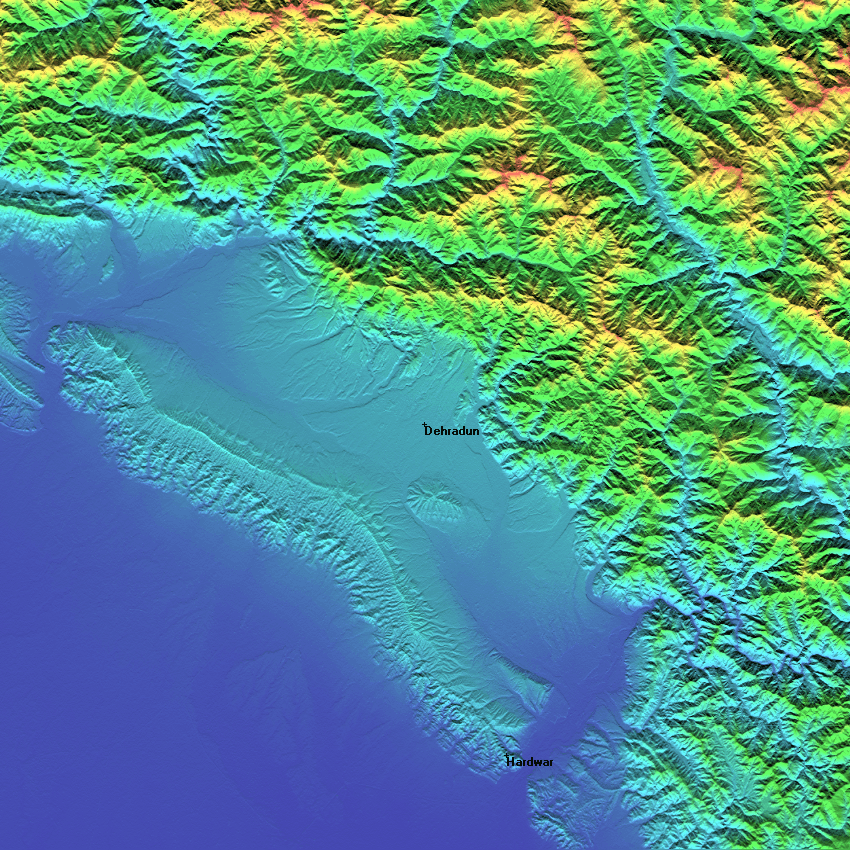
\includegraphics[width=0.35\textwidth]{Images/Dehradun, UK, IND.png}
    \caption{\small Target Area}
    \label{fig:TgrtDDN}
\end{wrapfigure}

By leveraging the natural topography of the Himalayan mountain range, these stations were positioned at altitudes of up to 3000 meters above sea level (figure \ref{fig:TgrtDDN}).
This approach significantly enhances signal propagation and extends coverage to areas that might otherwise be obstructed by terrain.

The figure \ref{fig:3Dpic} gives an idea about the microwave links and repeater positions in 3D space.
\begin{figure}[h!]
    \vspace{7mm}
    \centering
    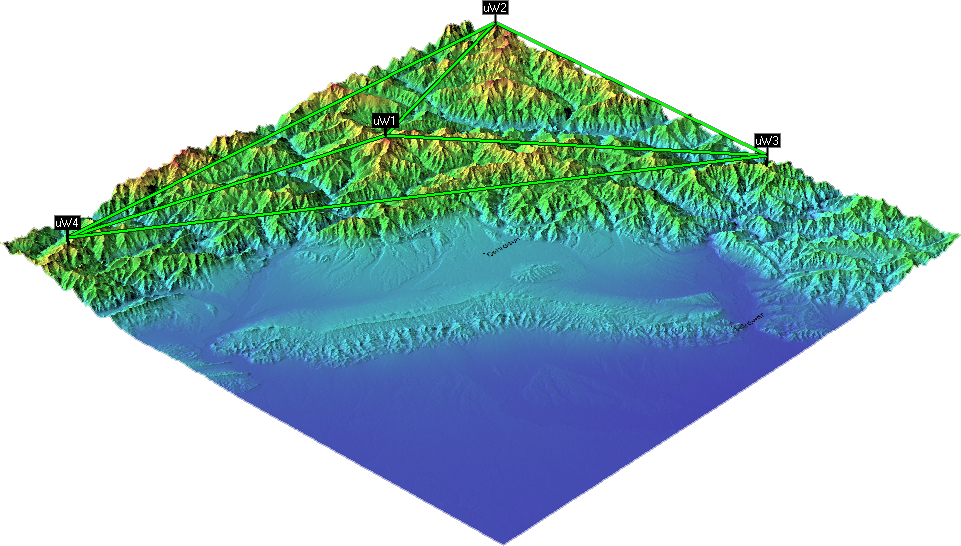
\includegraphics[width=0.9\textwidth]{Images/3D network.png}
    \caption{Microwave links of all repeaters \textit{in 3D}}
    \label{fig:3Dpic}
\end{figure}

Further details regarding the specific placement of the repeaters can be found below:
\begin{table}[h!]
    \centering
    \begin{tabular}{c c c c}
        \textbf{Unit Name} & \textbf{latitude} & \textbf{Longitude} & \textbf{Elevation}\\
        RP1 & 30$^\circ$35'15"N & 78$^\circ$09'00"E & 3007.9m\\
        RP2 & 30$^\circ$42'46"N & 78$^\circ$33'59"E & 3109.9m\\
        RP3 & 30$^\circ$09'53"N & 78$^\circ$30'53"E & 2244.9m\\
        RP4 & 30$^\circ$41'49"N & 77$^\circ$35'33"E & 2562.9m\\
    \end{tabular}
    \caption{Repeater details}
    \label{tab:repdel}
\end{table}

To visualise the coverage area of a specific unit, we can use the \textit{"Single Polar"} radio coverage plot.

It is accessed through the following steps:
\begin{enumerate}
    \item Go to the "Tools" menu
    \item Select "Radio Coverage"
    \item Choose "Single Polar"
\end{enumerate}
This will open a dedicated window where one can configure the plot settings and visualise the coverage area of the selected unit in a radial format.
The following images show the coverage area of individual repeaters (stations):

\begin{figure}[H]
\centering
        \begin{subfigure}[b]{0.45\textwidth}
            \centering
            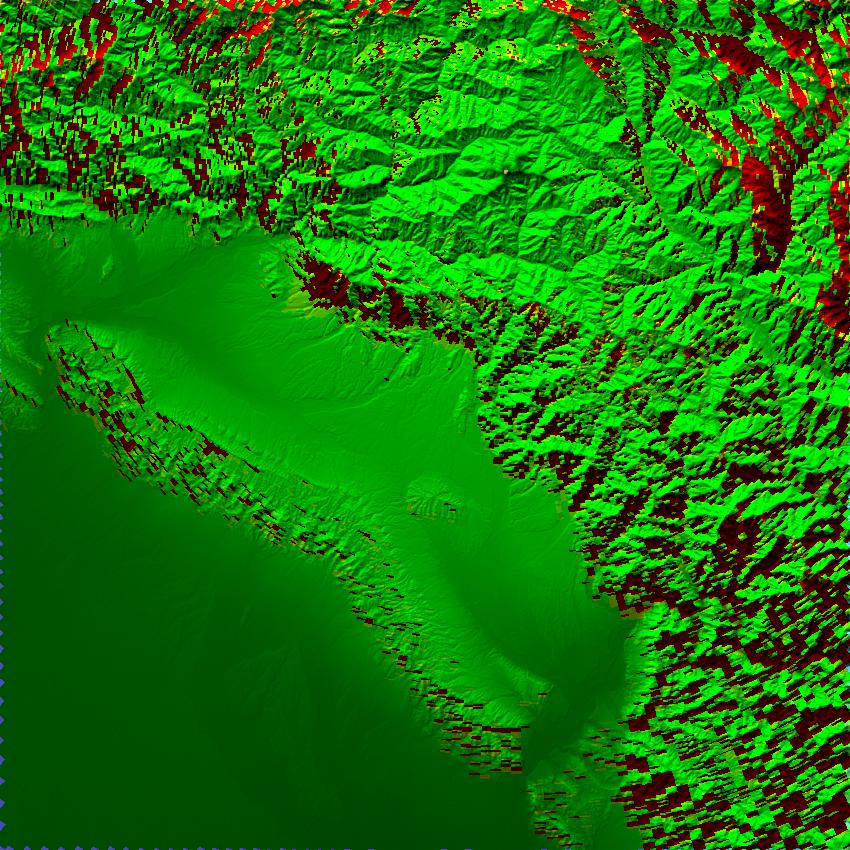
\includegraphics[width=\textwidth]{Images/RP1 Coverage.jpg}
            \caption{\small RP1}    
            \label{fig:RP1}
        \end{subfigure}
        \hfill
        \begin{subfigure}[b]{0.45\textwidth}
            \centering
            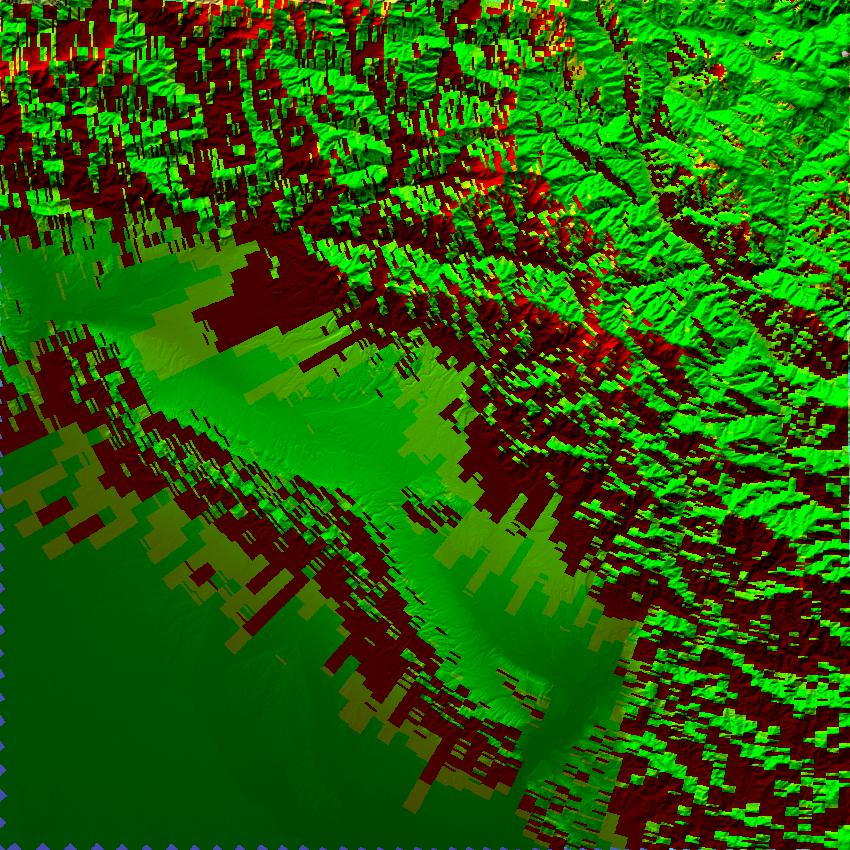
\includegraphics[width=\textwidth]{Images/RP2 Coverage.jpg}
            \caption{RP2}    
            \label{fig:RP2}
        \end{subfigure}
        \vskip\baselineskip
        \begin{subfigure}[b]{0.45\textwidth}
            \centering
            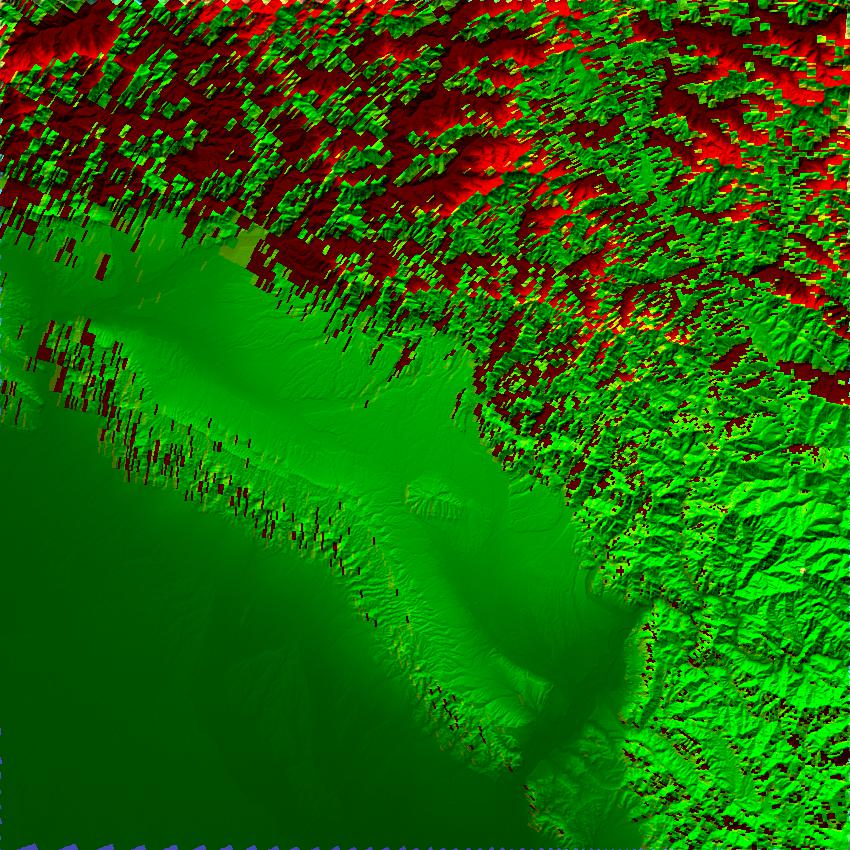
\includegraphics[width=\textwidth]{Images/RP3 Coverage.jpg}
            \caption{\small RP3}    
            \label{fig:RP3}
        \end{subfigure}
        \hfill
        \begin{subfigure}[b]{0.45\textwidth}
            \centering
            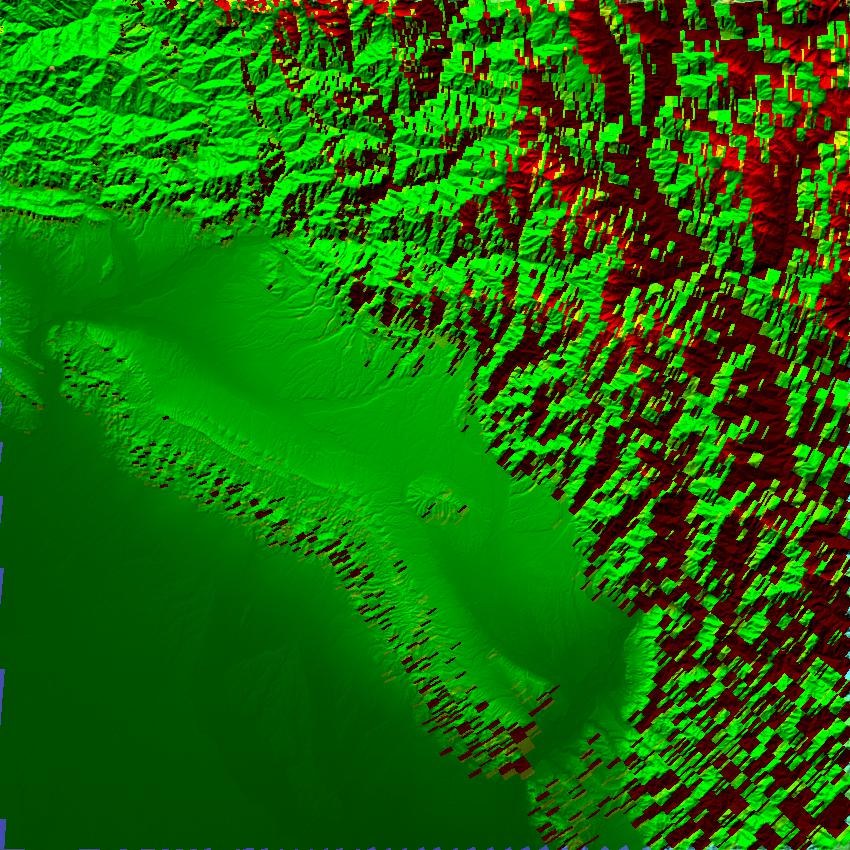
\includegraphics[width=\textwidth]{Images/RP4 Coverage.jpg}
            \caption{\small RP4}    
            \label{fig:RP4}
        \end{subfigure}
        \caption{Single Polar Radio Coverage for all repeaters} 
        \label{fig:IndNetCov}
\end{figure}

\subsubsection{Combined coverage}
To generate a \textit{"Combined Cartesian Radio Coverage"} plot in RadioMobile, follow these steps:
\begin{enumerate}
    \item \textbf{Select Units}: In the \textit{"Units"} tab, choose all repeaters to visualise the combined signal strength from all fixed units.
    \item \textbf{Mobile Unit Selection}: In the \textit{"Mobile Unit"} tab, select the previously defined \textit{"Mobile\_unit"} unit. This specifies the receiver for which the coverage is being calculated.
    \item \textbf{Network Selection}: In the \textit{"Network"} tab, choose the \textit{"VHF\_163MHz"} network which will cover the plot only considering the signal strength within the VHF network.
    \item \textbf{Units and Draw Size}:
    \begin{itemize}
        \item \textit{Units}: Select "dBm" as the desired unit for displaying signal strength on the plot.
        \item \textit{Draw Size}: Set the \textit{"Draw Size (pixel)"} to 2 to ensure maximum detail and accuracy in the coverage plot.
    \end{itemize}
    \item \textbf{Generate Plot}: Click the \textit{"DRAW"} button to generate the combined Cartesian radio coverage plot.
\end{enumerate}
\begin{figure}[h]
    \centering
    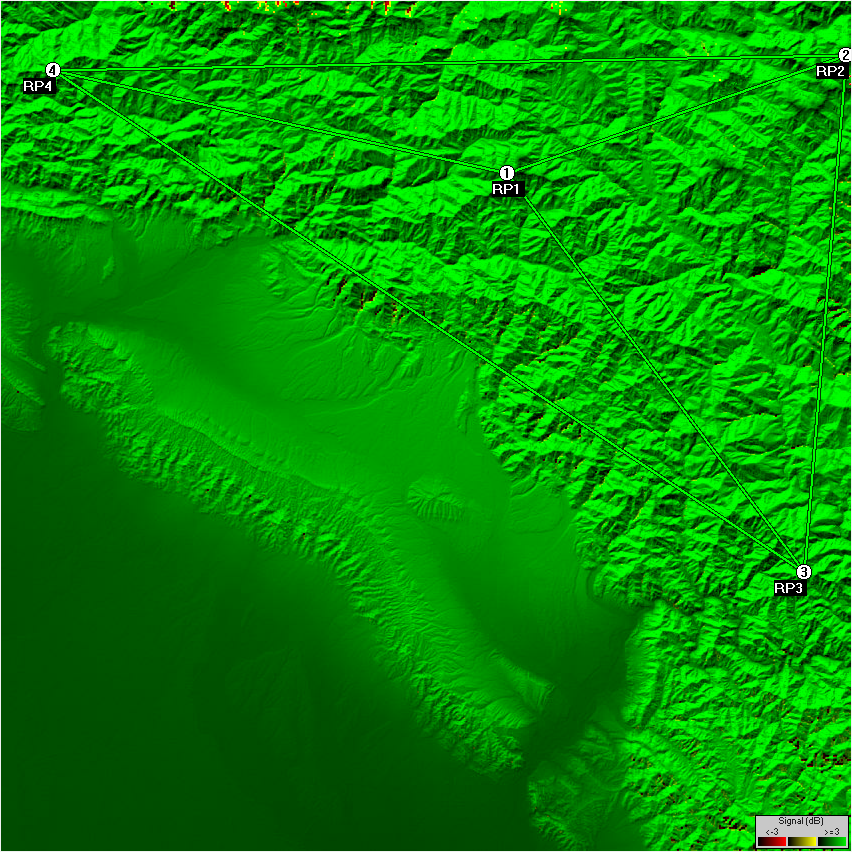
\includegraphics[width=0.75\textwidth]{Images/Final area coverage.png}
    \caption{Combined cartesian radio coverage with links and position of repeaters}
    \label{fig:CCradCov}
\end{figure}

\subsection{Link Analysis}
\subsubsection{Radio links}
To ensure optimal performance and reliability of radio links, it's crucial to maintain a clear line-of-sight path between the transmitting and receiving antennas.
This means that any potential obstructions should be minimised or eliminated along the direct path of the radio signal.
According to the project guidelines, we strictly adhere to maintaining an unobstructed line-of-sight to enhance the effectiveness of our radio network.

\begin{figure}[H]
\centering
        \begin{subfigure}[b]{0.45\textwidth}
            \centering
            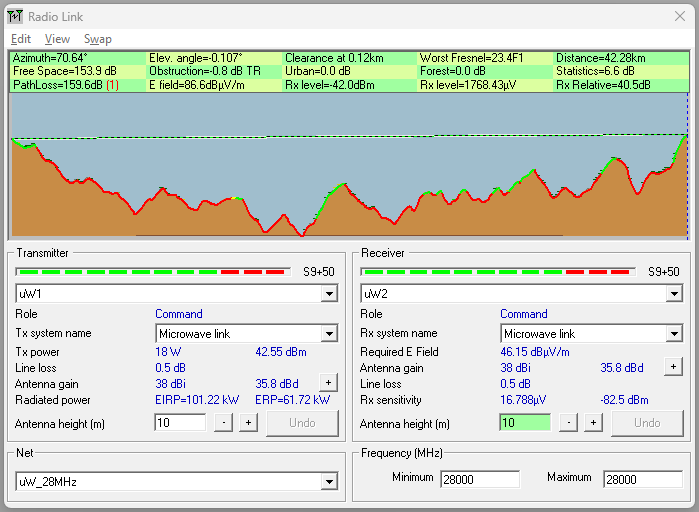
\includegraphics[width=\textwidth]{Images/uWL1-2.png}
            \caption{\small RP1 and RP2}    
            \label{fig:RP1-RP2}
        \end{subfigure}
        \hfill
        \begin{subfigure}[b]{0.45\textwidth}
            \centering
            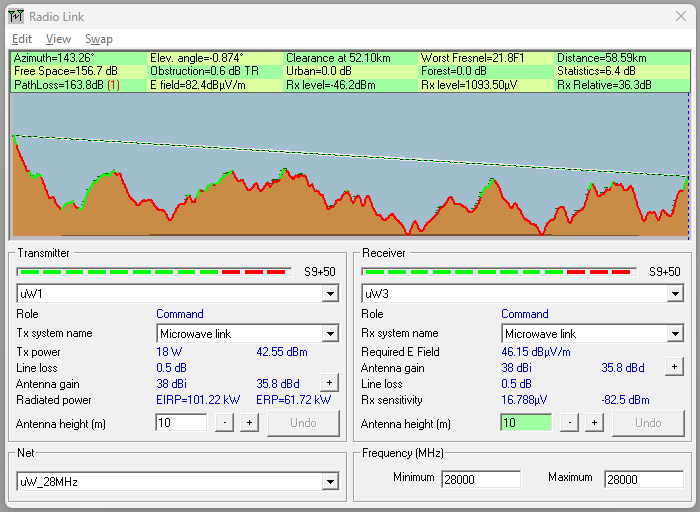
\includegraphics[width=\textwidth]{Images/uWL1-3.png}
            \caption{RP1 and RP3}    
            \label{fig:RP1-RP3}
        \end{subfigure}
        \vskip\baselineskip
        \begin{subfigure}[b]{0.45\textwidth}
            \centering
            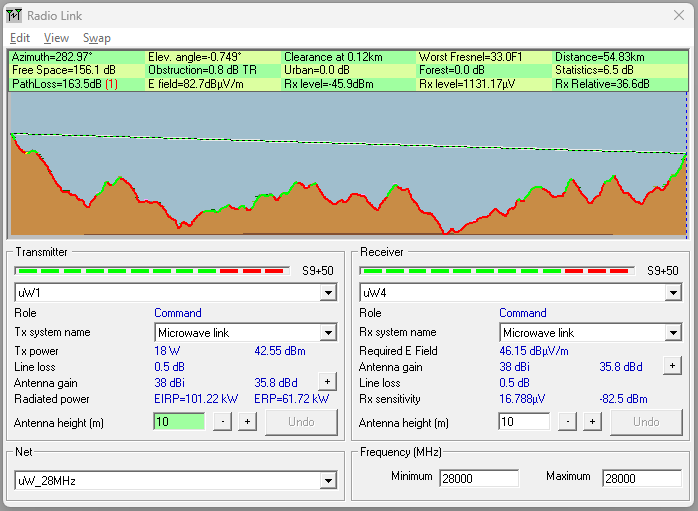
\includegraphics[width=\textwidth]{Images/uWL1-4.png}
            \caption{\small RP1 and RP4}    
            \label{fig:RP1-RP4}
        \end{subfigure}
        \hfill
        \begin{subfigure}[b]{0.45\textwidth}
            \centering
            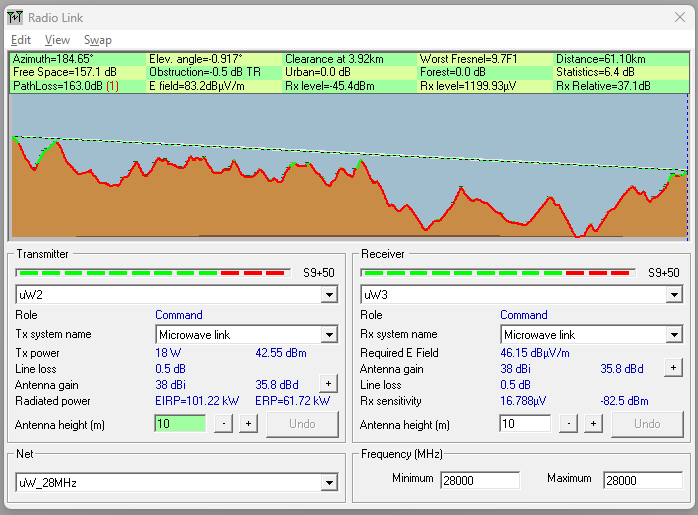
\includegraphics[width=\textwidth]{Images/uWL2-3.png}
            \caption{\small RP2 and RP3}    
            \label{fig:RP2-RP3}
        \end{subfigure}
        \vskip\baselineskip
        \begin{subfigure}[b]{0.45\textwidth}
            \centering
            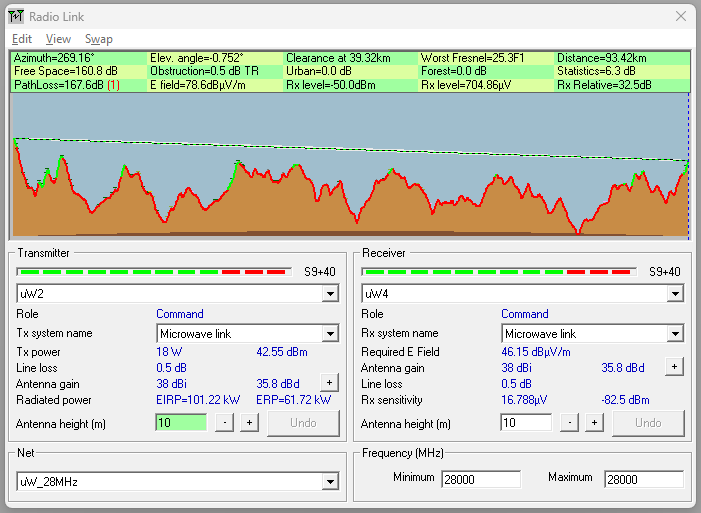
\includegraphics[width=\textwidth]{Images/uWL2-4.png}
            \caption{\small RP2 and RP4}    
            \label{fig:RP2-RP4}
        \end{subfigure}
        \hfill
        \begin{subfigure}[b]{0.45\textwidth}
            \centering
            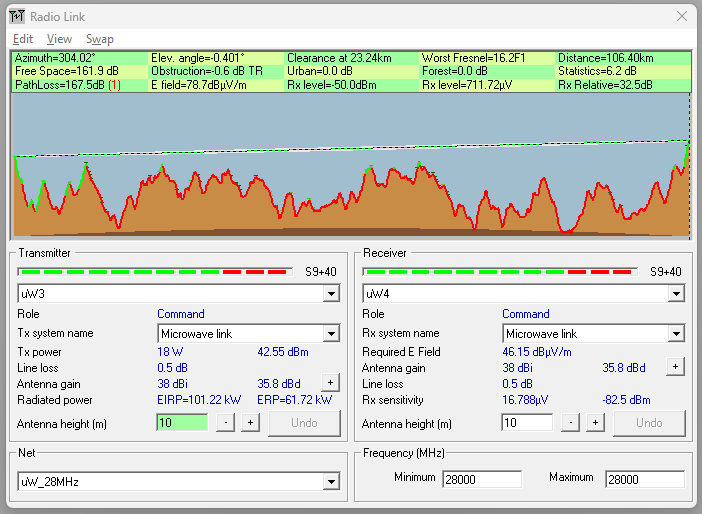
\includegraphics[width=\textwidth]{Images/uWL3-4.png}
            \caption{\small RP3 and RP4}    
            \label{fig:RP3-RP4}
        \end{subfigure}
        \caption{Microwave links between all repeaters} 
        \label{fig:IndNetCov}
\end{figure}

\subsubsection{Network report}
The \textit{"Network Report"} tool in Radio Mobile provides valuable insights into the overall health and performance of the network.
In this case, it generates a symmetric matrix where each number represents the quality of a specific point-to-point link between repeaters.
The quality of each link is assessed and represented using a specific pattern: \textbf{50 + signal margin in dB}.

Therefore, any value exceeding 50 indicates a robust and reliable radio link.
To ensure optimal routing the antenna directions were meticulously chosen to guarantee that all repeaters are visible from each individual repeater station.
\begin{figure}[h]
    \centering
    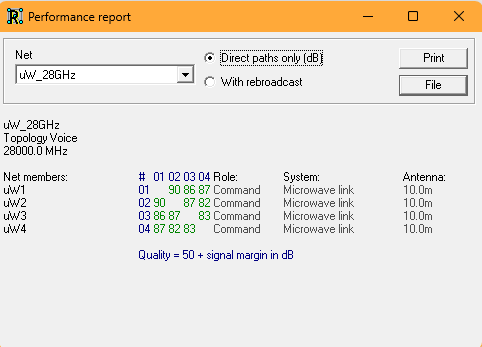
\includegraphics[width=0.75\textwidth]{Images/Performance Report.png}
    \caption{Performance report of the 28GHz microwave network}
    \label{fig:Perfrep}
\end{figure}

As depicted in the provided figure, all repeaters in the network have clear line-of-sight visibility to each other.


\subsubsection{Image analysis for area coverage}

\begin{wrapfigure}[]{r}{0.45\textwidth}
    \vspace{-5mm}
    \centering
    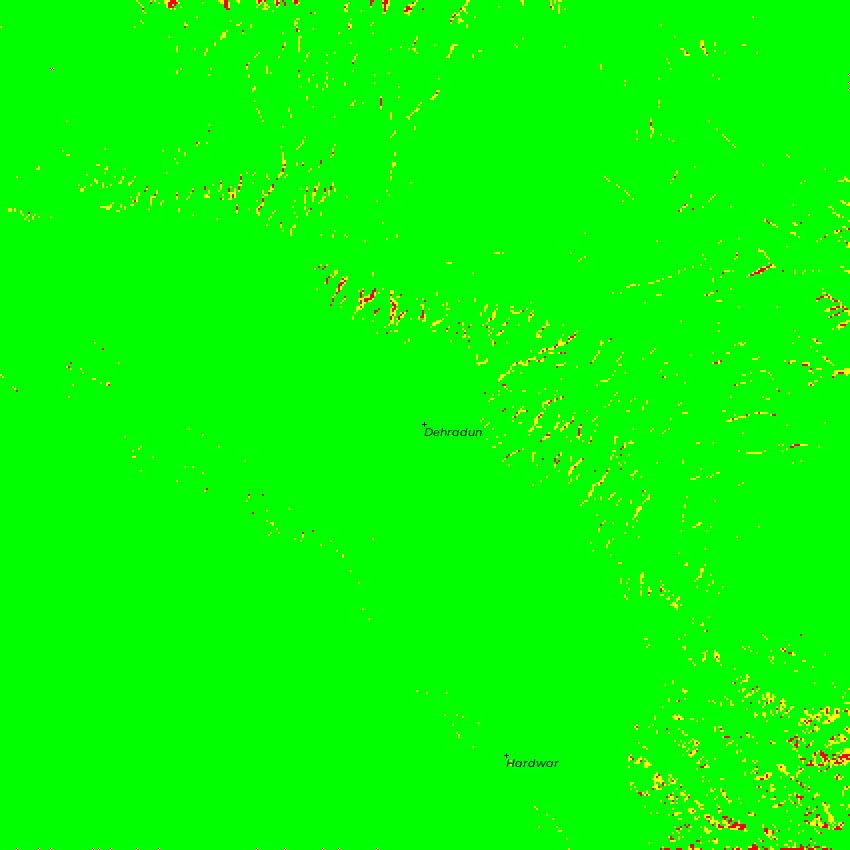
\includegraphics[width=0.35\textwidth]{Images/Combined.jpg}
    \caption{\small Image used for area analysis}
    \label{fig:ImgAna}
\end{wrapfigure}
To accurately determine the total area covered by the radio network, the map was reloaded with a white background.
This provided a clean and uncluttered image for analysis, followed by the combined coverage simulation without any legends, ensuring only the essential signal strength data was displayed.

To determine the area covered by the radio network, a Python script was utilised (refer to \ref{AppA}).
This script employed the {\fontfamily{cmtt}\selectfont extcolors} package to perform pixel-by-pixel analysis of the coverage image.
\par
